\documentclass[10pt,A4,english]{article}	



% we use utf8 since we want to build from any machine
\usepackage[utf8]{inputenc}		
\usepackage[USenglish]{isodate}
\usepackage{fancyhdr}
\usepackage[numbers]{natbib}
\usepackage{hyperref}

\hypersetup{
    colorlinks=true,
    linkcolor=blue,  
    urlcolor=cyan
    }


% provides \isempty test
\usepackage{xstring, xifthen}
\usepackage{enumitem}
\usepackage[english, russian]{babel}
\usepackage{blindtext}
\usepackage{pdfpages}
\usepackage{changepage}


% some tex-live fonts - choose your own

%\usepackage[defaultsans]{droidsans}
%\usepackage[default]{comfortaa}
%\usepackage{cmbright}
\usepackage[default]{raleway}
%\usepackage{fetamont}
%\usepackage[default]{gillius}
%\usepackage[light,math]{iwona}
%\usepackage[thin]{roboto} 

% set font default
\renewcommand*\familydefault{\sfdefault} 	
\usepackage[T1]{fontenc}

% more font size definitions
\usepackage{moresize}

\newcommand{\MYhref}[3][blue]{\href{#2}{\color{#1}{#3}}}%

% include the fontawesome icon set
\usepackage{fontawesome}

% use to vertically center content
% credits to: http://tex.stackexchange.com/questions/7219/how-to-vertically-center-two-images-next-to-each-other
\newcommand{\vcenteredinclude}[1]{\begingroup
\setbox0=\hbox{\includegraphics{#1}}%
\parbox{\wd0}{\box0}\endgroup}
\newcommand{\tab}[1]{\hspace{.2\textwidth}\rlap{#1}}
% use to vertically center content
% credits to: http://tex.stackexchange.com/questions/7219/how-to-vertically-center-two-images-next-to-each-other
\newcommand*{\vcenteredhbox}[1]{\begingroup
\setbox0=\hbox{#1}\parbox{\wd0}{\box0}\endgroup}

% icon shortcut
\newcommand{\icon}[3] { 							
	\makebox(#2, #2){\textcolor{maincol}{\csname fa#1\endcsname}}
}	


% icon with text shortcut
\newcommand{\icontext}[4]{ 						
	\vcenteredhbox{\icon{#1}{#2}{#3}}  \hspace{2pt}  \parbox{0.9\mpwidth}{\textcolor{#4}{#3}}
}

% icon with website url
\newcommand{\iconhref}[5]{ 						
    \vcenteredhbox{\icon{#1}{#2}{#5}}  \hspace{2pt} \href{#4}{\textcolor{#5}{#3}}
}

% icon with email link
\newcommand{\iconemail}[5]{ 						
    \vcenteredhbox{\icon{#1}{#2}{#5}}  \hspace{2pt} \href{mailto:#4}{\textcolor{#5}{#3}}
}

\usepackage{fontawesome}
\usepackage{setspace}

%----------------------------------------------------------------------------------------
%	PAGE LAYOUT  DEFINITIONS
%----------------------------------------------------------------------------------------

% page outer frames (debug-only)
% \usepackage{showframe}		

% we use paracol to display breakable two columns
\usepackage{paracol}
\usepackage{tikzpagenodes}
\usetikzlibrary{calc}
\usepackage{lmodern}
\usepackage{multicol}
\usepackage{lipsum}
\usepackage{atbegshi}
% define page styles using geometry
\usepackage[a4paper]{geometry}

% remove all possible margins
\geometry{top=1cm, bottom=1cm, left=1cm, right=1cm}

\usepackage{fancyhdr}
\pagestyle{empty}

% space between header and content
% \setlength{\headheight}{0pt}

% indentation is zero
\setlength{\parindent}{0mm}

%----------------------------------------------------------------------------------------
%	TABLE /ARRAY DEFINITIONS
%---------------------------------------------------------------------------------------- 

% extended aligning of tabular cells
\usepackage{array}

% custom column right-align with fixed width
% use like p{size} but via x{size}
\newcolumntype{x}[1]{%
>{\raggedleft\hspace{0pt}}p{#1}}%


%----------------------------------------------------------------------------------------
%	GRAPHICS DEFINITIONS
%---------------------------------------------------------------------------------------- 

%for header image
\usepackage{graphicx}

% use this for floating figures
% \usepackage{wrapfig}
% \usepackage{float}
% \floatstyle{boxed} 
% \restylefloat{figure}

%for drawing graphics		
\usepackage{tikz}			
\usepackage{ragged2e}	
\usetikzlibrary{shapes, backgrounds,mindmap, trees}

%----------------------------------------------------------------------------------------
%	Color DEFINITIONS
%---------------------------------------------------------------------------------------- 
\usepackage{transparent}
\usepackage{color}

% primary color
\definecolor{maincol}{RGB}{64,64,64}

% accent color, secondary
% \definecolor{accentcol}{RGB}{ 250, 150, 10 }

% dark color
\definecolor{darkcol}{RGB}{ 70, 70, 70 }

% light color
\definecolor{lightcol}{RGB}{245,245,245}

\definecolor{accentcol}{RGB}{0,87,87}



% Package for links, must be the last package used
\usepackage{hyperref}

% returns minipage width minus two times \fboxsep
% to keep padding included in width calculations
% can also be used for other boxes / environments
\newcommand{\mpwidth}{\linewidth-\fboxsep-\fboxsep}
	


%============================================================================%
%
%	CV COMMANDS
%
%============================================================================%

%----------------------------------------------------------------------------------------
%	 CV LIST
%----------------------------------------------------------------------------------------

% renders a standard latex list but abstracts away the environment definition (begin/end)
\newcommand{\cvlist}[1] {
	\begin{itemize}{#1}\end{itemize}
}

%----------------------------------------------------------------------------------------
%	 CV TEXT
%----------------------------------------------------------------------------------------

% base class to wrap any text based stuff here. Renders like a paragraph.
% Allows complex commands to be passed, too.
% param 1: *any
\newcommand{\cvtext}[1] {
	\begin{tabular*}{1\mpwidth}{p{0.98\mpwidth}}
		\parbox{1\mpwidth}{#1}
	\end{tabular*}
}
\newcommand{\cvtextsmall}[1] {
	\begin{tabular*}{0.8\mpwidth}{p{0.8\mpwidth}}
		\parbox{0.8\mpwidth}{#1}
	\end{tabular*}
}
%----------------------------------------------------------------------------------------
%	CV SECTION
%----------------------------------------------------------------------------------------

% Renders a a CV section headline with a nice underline in main color.
% param 1: section title
\newcommand{\cvsection}[1] {
	\vspace{14pt}
	\cvtext{
		\textbf{\LARGE{\textcolor{darkcol}{#1}}}\\[-4pt]
		\textcolor{accentcol}{ \rule{0.2\textwidth}{1.5pt} } \\
	}
}

\newcommand{\cvsectionsmall}[1] {
	\vspace{14pt}
	\cvtext{
		\textbf{\Large{\textcolor{darkcol}{#1}}}\\[-4pt]
		\textcolor{accentcol}{ \rule{0.2\textwidth}{1.5pt} } \\
	}
}

\newcommand{\cvheadline}[1] {
	\vspace{16pt}
	\cvtext{
		\textbf{\Huge{\textcolor{accentcol}{#1}}}\\[-4pt]
		 
	}
}

\newcommand{\cvsubheadline}[1] {
	\vspace{16pt}
	\cvtext{
		\textbf{\huge{\textcolor{darkcol}{#1}}}\\[-4pt]
		 
	}
}
%----------------------------------------------------------------------------------------
%	META SKILL
%----------------------------------------------------------------------------------------

% Renders a progress-bar to indicate a certain skill in percent.
% param 1: name of the skill / tech / etc.
% param 2: level (for example in years)
% param 3: percent, values range from 0 to 1
\newcommand{\cvskill}[3] {
	\begin{tabular*}{1\mpwidth}{p{0.72\mpwidth}  r}
 		\textcolor{black}{\textbf{#1}} & \textcolor{maincol}{#2}\\
	\end{tabular*}%
	
	\hspace{4pt}
	\begin{tikzpicture}[scale=1,rounded corners=2pt,very thin]
		\fill [lightcol] (0,0) rectangle (1\mpwidth, 0.15);
		\fill [accentcol] (0,0) rectangle (#3\mpwidth, 0.15);
  	\end{tikzpicture}%
}


%----------------------------------------------------------------------------------------
%	 CV EVENT
%----------------------------------------------------------------------------------------

% Renders a table and a paragraph (cvtext) wrapped in a parbox (to ensure minimum content
% is glued together when a pagebreak appears).
% Additional Information can be passed in text or list form (or other environments).
% the work you did
% param 1: time-frame i.e. Sep 14 - Jan 15 etc.
% param 2:	 event name (job position etc.)
% param 3: Customer, Employer, Industry
% param 4: Short description
% param 5: work done (optional)
% param 6: technologies include (optional)
% param 7: achievements (optional)
\newcommand{\cvevent}[7] {
	
	% we wrap this part in a parbox, so title and description are not separated on a pagebreak
	% if you need more control on page breaks, remove the parbox
	\parbox{\mpwidth}{
		\begin{tabular*}{1\mpwidth}{p{0.66\mpwidth}  r}
	 		\textcolor{black}{\textbf{#2}} & \colorbox{accentcol}{\makebox[0.32\mpwidth]{\textcolor{white}{\textbf{#1}}}} \\
			\textcolor{maincol}{#3} & \\
		\end{tabular*}\\[8pt]
	
		\ifthenelse{\isempty{#4}}{}{
			\cvtext{#4}\\
		}
	}
	\vspace{14pt}
}


%----------------------------------------------------------------------------------------
%	 CV META EVENT
%----------------------------------------------------------------------------------------

% Renders a CV event on the sidebar
% param 1: title
% param 2: subtitle (optional)
% param 3: customer, employer, etc,. (optional)
% param 4: info text (optional)
\newcommand{\cvmetaevent}[4] {
	\textcolor{maincol} { \cvtext{\textbf{\begin{flushleft}#1\end{flushleft}}}}

	\ifthenelse{\isempty{#2}}{}{
	\textcolor{black} {\cvtext{\textbf{#2}} }
	}

	\ifthenelse{\isempty{#3}}{}{
		\cvtext{{ \textcolor{maincol} {#3} }}\\
	}

	\cvtext{#4}\\[14pt]
}

%---------------------------------------------------------------------------------------
%	QR CODE
%----------------------------------------------------------------------------------------

% Renders a qrcode image (centered, relative to the parentwidth)
% param 1: percent width, from 0 to 1
\newcommand{\cvqrcode}[1] {
	\begin{center}
		\includegraphics[width={#1}\mpwidth]{qrcode}
	\end{center}
}


% HEADER AND FOOOTER 
%====================================
\newcommand\Header[1]{%
\begin{tikzpicture}[remember picture,overlay]
\fill[accentcol]
  (current page.north west) -- (current page.north east) --
  ([yshift=50pt]current page.north east|-current page text area.north east) --
  ([yshift=50pt,xshift=-3cm]current page.north|-current page text area.north) --
  ([yshift=10pt,xshift=-5cm]current page.north|-current page text area.north) --
  ([yshift=10pt]current page.north west|-current page text area.north west) -- cycle;
\node[font=\sffamily\bfseries\color{white},anchor=west,
  xshift=0.7cm,yshift=-0.32cm] at (current page.north west)
  {\fontsize{12}{12}\selectfont {#1}};
\end{tikzpicture}%
}

\newcommand\Footer[1]{%
\begin{tikzpicture}[remember picture,overlay]
\fill[lightcol]
  (current page.south east) -- (current page.south west) --
  ([yshift=-80pt]current page.south east|-current page text area.south east) --
  ([yshift=-80pt,xshift=-6cm]current page.south|-current page text area.south) --
  ([xshift=-2.5cm,yshift=-10pt]current page.south|-current page text area.south) --	
  ([yshift=-10pt]current page.south east|-current page text area.south east) -- cycle;
\node[yshift=0.32cm,xshift=9cm] at (current page.south) {\fontsize{10}{10}\selectfont \textbf{\thepage}};
\end{tikzpicture}%
}


%=====================================
%============================================================================%
%
%
%
%	DOCUMENT CONTENT
%
%
%
%============================================================================%
\begin{document}

\columnratio{0.31}
\setlength{\columnsep}{2.2em}
\setlength{\columnseprule}{4pt}
\colseprulecolor{white}


% LEBENSLAUF HIERE
\AtBeginShipoutFirst{\Header{Резюме}\Footer{1}}
\AtBeginShipout{\AtBeginShipoutAddToBox{\Header{Резюме}\Footer{2}}}

\newpage

\colseprulecolor{lightcol}
\columnratio{0.31}
\setlength{\columnsep}{2.2em}
\setlength{\columnseprule}{4pt}
\begin{paracol}{2}


\begin{leftcolumn}
%---------------------------------------------------------------------------------------
%	META IMAGE
%----------------------------------------------------------------------------------------
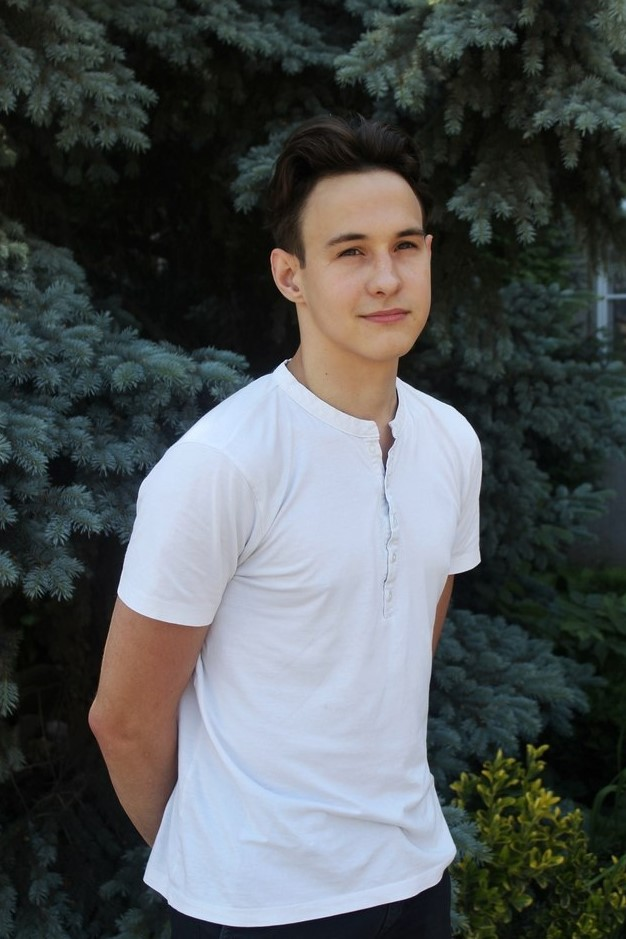
\includegraphics[width=\linewidth]{resources/image.jpg}	%trimming relative to image size

%---------------------------------------------------------------------------------------
%	META SKILLS
%----------------------------------------------------------------------------------------
	\fcolorbox{white}{white}{\begin{minipage}[c][1cm][c]{1\mpwidth}
		\LARGE{\textbf{\textcolor{maincol}{Максим Пешков}}} 
\end{minipage}} \\
\icontext{CaretRight}{12}{22 года}{black}\\[2pt]
\icontext{CaretRight}{12}{4 курс бакалавриата}{black}\\[2pt]

\vspace{-0.5cm}

\cvsection{Контакты}

\vspace{-0.2cm}
\icontext{MapMarker}{16}{Москва}{black}\\[2pt]
\icontext{MobilePhone}{16}{+7(918)625-83-92}{black}\\[2pt]
\iconemail{Envelope}{16}{myupeshkov@gmail.com}{myupeshkov@gmail.com}{black}\\[2pt]
\iconhref{Github}{16}{github.com/myupeshkov}{https://github.com/myupeshkov}{black}\\[2pt]
\- \- \faLinkedinSquare \MYhref[black]{https://www.linkedin.com/in/maksim-peshkov-973374234/}{ \hspace{0.35cm} LinkedIn (Maksim Peshkov)}


\vspace{-0.2cm}


\cvsection{Навыки}

\cvskill{Python (numpy, pandas, sklearn, pytorch)} {} {0.9} \\[-0.3pt]

\vspace{-10pt}

\cvskill{MS Office (Excel)} {} {0.75} \\[-0.5pt]

\vspace{-10pt}

\cvskill{R} {} {0.7} \\[-1pt]

\vspace{-10pt}

\cvskill{SQL} {} {0.8} \\[-1pt]

\vspace{-10pt}

\cvskill{STATA} {} {0.7} \\[-1pt]

\vspace{-10pt}

\cvskill{Теория вероятности и статистика} {} {0.92} \\[-1pt]

\vspace{-10pt}

\cvskill{Эконометрика} {} {0.92} \\[-1pt]

\vspace{-10pt}

\cvskill{Data Science} {} {0.8} \\[-1pt]

\vspace{-10pt}

\cvskill{Machine learning/ \newline Deep learning} {} {0.8} \\[-1pt]

\cvskill{Русский}{родной} {1} \\[-1pt]

\vspace{-10pt}

\cvskill{English} {B2} {0.7} \\[-1pt]

\newpage
%---------------------------------------------------------------------------------------
%	EDUCATION
%----------------------------------------------------------------------------------------


\cvsection{Интересы}

\icontext{CaretRight}{12}{Data Science}{black}\\[6pt]
\icontext{CaretRight}{12}{Эконометрика}{black}\\[6pt]
\icontext{CaretRight}{12}{Институциональная \newline экономика}{black}\\[6pt]
\icontext{CaretRight}{12}{Интеллектуальные игра \newline "Что? Где? Когда?"{}}{black}\\[6pt]
\icontext{CaretRight}{12}{Игра на гитаре}{black}\\[6pt]
	
%\cvqrcode{0.3}

\end{leftcolumn}
\begin{rightcolumn}
%---------------------------------------------------------------------------------------
%	TITLE  HEADER
%----------------------------------------------------------------------------------------


%---------------------------------------------------------------------------------------
%	PROFILE
%----------------------------------------------------------------------------------------



%---------------------------------------------------------------------------------------
%	WORK EXPERIENCE
%----------------------------------------------------------------------------------------

\vspace{10pt}
\cvsection{Образование}
\vspace{2pt}


\cvevent
{2018 - 2022}
	{НИУ "Высшая школа экономики" \hspace{1pt} | \hspace{1pt} г. Москва\newline Бакалавриат}
	{Факультет экономических наук \newline Экономика | GPA: 8,83 \newline
	Рейтинг: топ 2\% среди студентов бакалавриата}
	{Изучил на отлично курсы линейной алгебры, математического анализа, дифференциальных уравнений, случайных процессов, микро- и макроэкономики, теории вероятности и математической статистики, эконометрики.}
	\vfill\null

\vspace{-0.3cm}

\cvevent
{2019 - 2021}
	{НИУ "Высшая школа экономики" \hspace{1pt} | \hspace{1pt} г. Москва\newline Майнор}
	{Интеллектуальный анализ данных \newline ФКН | GPA: 9}
	{В рамках майнора изучил современные методы машинного обучения в Python, методы работы с текстовыми данными, основы глубинного обучения (основные архитектуры и обучение нейронных сетей). Более подробно см. \href{https://github.com/myupeshkov/Machine_Learning}{здесь} и \href{https://github.com/myupeshkov/Deep_Learning}{здесь}.}
	\vfill\null
	
\vspace{-0.3cm}

\cvevent
{2007 - 2018}
	{МОУ Гимназия №87 \hspace{1pt} | \hspace{1pt} г. Краснодар}
	{Среднее общее и основное общее образование закончил с красными аттестатами}{}
	\vfill\null
	
\vspace{-1cm}	

\cvsection{Опыт работы}

\cvevent
{03/2020 - н.э.}
	{Стажер-исследователь}
	{Институт институциональных исследований\newline НИУ ВШЭ}
	{Анализ экономических институтов в регионах России и выявление факторов их развития. Сбор, обработка и визуализация данных в  Python. Построение эконометрических моделей и проверка гипотез.}
	\vfill\null


\cvevent
{01/2021 - 06/2021}
	{Ассистент курса "Анализ данных на Python"}
	{Факультет компьютерных наук\newline НИУ ВШЭ}
	{Проведение консультаций и устных опросов по алгоритмическим задачам на языке Python.}
	\vfill\null
	

\cvevent
{06/2021 - 12/2021}
	{Младший продуктовый аналитик}
	{Департамент товарного кредитования \newline АО "Тинькофф банк'}
	{Анализ продуктовых метрик, выявление слабых сторон POS-кредитования, предложение улучшения Tinkoff Credit Broker, проверка статистических гипотез при помощи А/В тестирования.}
	\vfill\null

\vspace{-0.5cm}

\cvsection{Проектная деятельность}

\cvevent
{02/2020 - 06/2020}
	{Учебный проект "Модельный риск" \hspace{1pt} | \hspace{1pt} г. Москва}
	{Лаборатория по финансовой инженерии\newline и риск-менеджменту\newline НИУ ВШЭ}
	{Анализ российского рынка государственных облигаций, использование различных моделей для построения кривой доходности, измерение модельного риска в зависимости от используемого подхода заполнения пропуска: Фильтр Калмана, EM-алгоритм, Random Forest и другие. Более подробно описано \href{https://github.com/myupeshkov/Model_risk}{здесь}.
	}
	\vfill\null

\vspace{-0.3cm}

\cvevent
{02/2020 - 05/2020}
	{Проект "Перспективы развития инфраструктуры российского финансового рынка"  \hspace{1pt} | \hspace{1pt} г. Москва}
	{Национальный расчетный депозитарий}	
	{Анализ практик использования технологии блокчейн на зарубежных валютных биржах, оценка технологических и финансовых рисков,  разработка аналога для российского рынка.
	Более подробно описано \href{https://github.com/myupeshkov/NSD_MOEX}{здесь}.
	}
	\vfill\null


\vspace{-0.6cm}

\cvsection{Конференции}
\begin{itemize}
    \item 2021-2022
    \begin{itemize}
        \item Докладчик "Санкт-Петербургской международной конференции по неравенству и многообразию". Более подробно см. \href{https://spb.hse.ru/en/idc/#about}{здесь}
        
    \item Докладчик в конференции Национального расчетного депозитария (группа "Московская биржа") "Будущее финансовой инфраструктуры"{}. Более подробно см. \href{https://github.com/myupeshkov/NSD_MOEX/tree/main/conference_2021}{здесь}.
    \end{itemize}
    
\end{itemize}

\vspace{-0.3cm}


\cvsection{Олимпиады}

\vspace{-0.35cm}
\begin{itemize}
\item 2021-2022
\vspace{-0.1cm}
\begin{itemize}

    \item Призер олимпиады "Econometrics Universiade"{}. Более подробно см. \href{https://new.universiade-ecm.com/results/}{здесь}
    \item Участник заключительного этапа олимпиады "Я-Профи"{} по направлениям "Математика"{}, "Бизнес-информатика"{}, "Математическое моделирование"{}
    \item Участник заключительного этапа олимпиады "Высшая лига" по направлениям "Бизнес-информатика", "Прикладная математика"{}, "Экономика"{}
    \item Участник заключительного этапа олимпиады "МегаОлимпиада" университета ИТМО по направлению "Математическое моделирование"{} трека "Информационные системы"{}
    
\end{itemize}

\item 2020-2021 
\vspace{-0.2cm}
\begin{itemize}

  \item Призер олимпиады "Высшая лига"{} по треку "Математические методы в экономике"{}
  
\end{itemize}

\item 2017-2018 года
\begin{itemize}
    \item Победитель регионального этапа Всероссийской олимпиады школьников по математике в 2017 и 2018 годах
    \item Призер олимпиады школьников СПбГУ по математике в 2018 году
    \item Участник заключительного этапа Всероссийской олимпиады школьников по математике в 2017 году
    \end{itemize}
\end{itemize}

\cvsection{Сертификаты}
\vspace{2pt}

\cvevent 
{03/2022 - 03/2024}
    {IELTS Academic}
    {Overall Band Score: 6.5 | CEFR level: B2}
    { }
\vfill\null

\vspace{-0.5cm}



% hofixes to create fake-space to ensure the whole height is used
\mbox{}
\vfill
\mbox{}
\vfill
\mbox{}
\vfill
\mbox{}
\vfill
\mbox{}
\vfill
\mbox{}
\vfill
\mbox{}

\end{rightcolumn}
\end{paracol}


\end{document}